\documentclass[12pt]{article}
%\usepackage[utf8]{inputenc}
%\documentclass[UTF8]{ctexart}
%\usepackage[UTF8, heading = false, scheme = plain]{ctex}
\usepackage{geometry}
%geometry{a4paper,scale=0.9}
\geometry{a4paper,left=1cm,right=1cm,top=1cm,bottom=2cm}
\usepackage{amsfonts}
\usepackage{color}
\usepackage{url}
%\usepackage{biblatex}
\usepackage{amsmath}
\usepackage{amssymb}
\usepackage{latexsym}
\usepackage{cite}
%\addbibresource{ref.bib}
%\bibliography{ref.bib}
\usepackage{caption}
\usepackage{graphicx, subfig}
\usepackage{float}
%\usepackage[fontset=ubuntu]{ctex}
%\usepackage{fontspec}
\usepackage{xeCJK}
%\usepackage[colorlinks,
%anchorcolor=black,
%citecolor=black]{hyperref}
%\setmainfont{SimSun}
\usepackage[section]{placeins}
\usepackage{enumitem}
\usepackage{framed}
\usepackage[framemethod=TikZ]{mdframed}
\usepackage{indentfirst}
\usepackage{setspace}%使用间距宏包
\linespread{1.5}
%\title{预备知识}
%\author{leolinuxer }
%\date{June 2020}

\title{模型效果的评估方法}
\author{leolinuxer}
%\date{June 2020}

\begin{document}
\maketitle
\tableofcontents

\section{评估目标的设定原则\cite{Deep_Learning_Recommender_System}}
以 YouTube 的推荐系统为例,推荐系统的终极优化目标应该包括两个维度:一个维度是用户体验的优化,另一个维度是满足公司的商业利益。对于 YouTube 公司而言,其优化用户体验结果的最直接体现就是用户观看时长的增加。而YouTube作为一家以广告位主要收入来源的公司,其商业利益也建立在用户观看时长的增长之上,因为总用户观看时长与广告的总曝光机会成正比。

所以,YouTube 推荐系统的优化目标就是用户观看时长,而不是传统系统看中的“点击率”。其大致推荐流程是:先通过构建深度学习模型,预测用户观看某候选视频的时长,再按照预测时长进行候选视频的排序,行成最终的推荐列表。

\section{各种率的定义}
\subsection{Confusion Matrix}
Confusion Matrix 矩阵如下表所示:

\begin{table}[h]
\begin{center}  
\begin{tabular}{|l|l|l|}  
\hline  
预测值-实际值 & True & False \\ \hline  
True &	True Positive(真阳性) &	False Positive(假阳性)\\  \hline
False &	False Negative(假阴性) & True Negative(真阴性)\\  \hline
\end{tabular}  
\end{center}
\caption{Confusion Matrix} 
\end{table}

\subsection{各种指标率}
正确率(Precision):
$$Precision = \frac{TP}{TP+FP}$$

真阳性率(True Positive Rate,TPR),灵敏度(Sensitivity),召回率(Recall):

$$Sensitivity = Recall= \frac{TP}{TP+FN}$$

真阴性率(True Negative Rate,TNR),特异度(Specificity):
$$Specificity = Recall= \frac{TN}{FP+TN}$$

假阴性率(False Negatice Rate,FNR),漏诊率( = 1 - 灵敏度):
$$ FNR = \frac{FN}{TP+FN}$$

假阳性率(False Positice Rate,FPR),误诊率( = 1 - 特异度):
$$ FPR = \frac{FP}{FP+TN}$$

\section{主要评价指标 \cite{ROC-AUC}}
\subsection{ROC}
对于分类器,或者说分类算法,评价指标主要有precision,recall,F-score等,以及这里要讨论的ROC和AUC。

ROC曲线:接收者操作特征曲线(receiver operating characteristic curve),是反映敏感性和特异性连续变量的综合指标,ROC曲线上每个点反映着对同一信号刺激的感受性。下图是一个ROC曲线的示例:

\begin{figure}[ht]
  \centering
  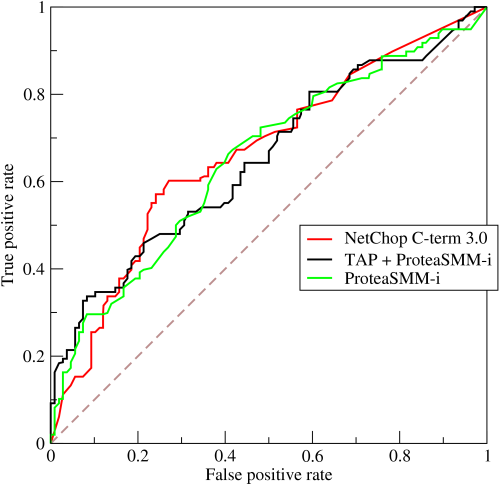
\includegraphics[width=.5\textwidth]{fig/ROC_example.png} %1.png是图片文件的相对路径
  \caption{ROC曲线示意} %caption是图片的标题
  \label{ROC_example} %此处的label相当于一个图片的专属标志,目的是方便上下文的引用
\end{figure}

ROC 曲线的横纵坐标分别为:

横坐标:1-Specificity,伪正类率(False positive rate, FPR),预测为正但实际为负的样本占所有负例样本的比例(负例中预测错了的比例);

纵坐标:Sensitivity,真正类率(True positive rate, TPR),预测为正且实际为正的样本占所有正例样本的比例(正例中预测对了的比例)。

在一个二分类模型中,假设采用逻辑回归分类器,其给出针对每个实例为正类的概率,那么通过设定一个阈值如0.6,概率大于等于0.6的为正类,小于0.6的为负类。对应的就可以算出一组(FPR,TPR),在平面中得到对应坐标点。随着阈值的逐渐减小,越来越多的实例被划分为正类,但是这些正类中同样也掺杂着真正的负实例,即TPR和FPR会同时增大。阈值最大时,对应坐标点为(0,0),阈值最小时,对应坐标点(1,1)。

\subsection{AUC(Area Under Curve)}
AUC (Area Under Curve) 被定义为ROC曲线下的面积,显然这个面积的数值不会大于1。又由于ROC曲线一般都处于y=x这条直线的上方(如果不是,那么可以交换阈值上下对应的分类,即可得到更好的分类结果),所以AUC的取值范围一般在0.5和1之间。使用AUC值作为评价标准是因为很多时候ROC曲线并不能清晰的说明哪个分类器的效果更好,而作为一个数值,对应AUC更大的分类器效果更好。

\subsection{为什么使用ROC曲线}
既然已经这么多评价标准(如precision-recall 等),为什么还要使用ROC和AUC呢?因为ROC曲线有个很好的特性:当测试集中的正负样本的分布变化的时候,ROC曲线能够保持不变。在实际的数据集中经常会出现类不平衡(class imbalance)现象,即负样本比正样本多很多(或者相反),而且测试数据中的正负样本的分布也可能随着时间变化。下图是ROC曲线和Precision-Recall曲线的对比:

\begin{figure}[ht]
  \centering
  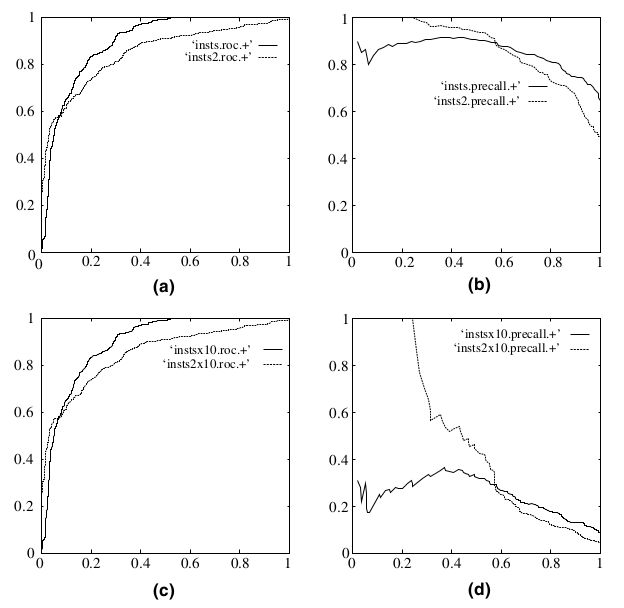
\includegraphics[width=.8\textwidth]{fig/ROC_vs_Precision_Recall.png} %1.png是图片文件的相对路径
  \caption{ROC vs Precision-Recall} %caption是图片的标题
  \label{ROC_vs_Precision_Recall} %此处的label相当于一个图片的专属标志,目的是方便上下文的引用
\end{figure}

在上图中,(a)和(c)为ROC曲线,(b)和(d)为Precision-Recall曲线。(a)和(b)展示的是分类其在原始测试集(正负样本分布平衡)的结果,(c)和(d)是将测试集中负样本的数量增加到原来的10倍后,分类器的结果。可以明显的看出,ROC曲线基本保持原貌,而Precision-Recall曲线则变化较大。

\subsection{平均精度均值(mAP, Mean Average Precision)}
平均精度均值是对平均精度(Average Precision)的再次平均。

要计算 mAP 必须先绘出各类别 PR 曲线,计算出 AP。假定推荐系统对某一用户测试集的排序结果如下表所示:
\begin{table}[h]
\begin{center}  
\begin{tabular}{|l|l|l|l|l|l|l|}  
\hline  
 推荐序列 & N = 1 & N= 2 & N=3 & N= 4 & N= 5 & N= 6 \\ \hline  
 真实标签 & 1 & 0 & 0 & 1 & 1 & 1 \\  \hline
\end{tabular}  
\end{center}
\end{table}

其中,1 代表正样本,0 代表负样本。

在排序模型中,通常没有一个确定的阈值把预测结果直接判定为正样本或负样本,而是采用 TopN 排序结果的精确率(precision@N)和召回率(recall@N)来衡量排序模型的性能,即认为模型排序的 TopN 的结果就是模型判定的正样本,然后计算 precision@N 和 recall@N。

接下来,计算上述序列中每个位置上的 precision@N:
\begin{table}[h]
\begin{center}  
\begin{tabular}{|l|l|l|l|l|l|l|}  
\hline  
 推荐序列 & N = 1 & N= 2 & N=3 & N= 4 & N= 5 & N= 6 \\ \hline  
 真实标签 & 1 & 0 & 0 & 1 & 1 & 1 \\  \hline
 precision@N & 1/1 & 1/2 & 1/3 & 2/4 & 3/5 & 4/6 \\  \hline
\end{tabular}  
\end{center}
\end{table}

AP 的计算只取正样本处的 precision 进行平均,即 AP = (1/1 + 2/4 + 3/5 + 4/6) = 0.6917,那么什么是 mAP 呢?

如果推荐系统对测试集中的每个用户都进行样本排序,那么每个用户都会计算出一个 AP 值,然后再对所有用户的 AP 值进行平均,就得到了 mAP。

值得注意的是,mAP 的计算方法和 P-R 曲线、ROC 曲线的计算方法完全不同,因为 mAP 需要对每个用户的样本进行分用户排序,而 P-R 曲线和 ROC 曲线均是对全量测试样本进行排序。

\subsection{精确率、准召率、F1 值 各自的优缺点\cite{Compare_P_R_F1_ROC_AUC}}

\subsubsection{精确率 Accuracy}
Accuracy 是最常见也是最基本的evaluation metric。但在binary classification 且正反例不平衡的情况下,尤其是我们对minority class 更感兴趣的时候,accuracy评价基本没有参考价值。什么fraud detection(欺诈检测),癌症检测,都符合这种情况。举个栗子:在测试集里,有100个sample,99个反例,只有1个正例。如果我的模型不分青红皂白对任意一个sample都预测是反例,那么我的模型的accuracy是正确的个数/总个数 = 99/100 = 99\%。你拿着这个accuracy高达99\%的模型屁颠儿屁颠儿的去预测新sample了,而它一个正例都分不出来,有意思么……也有人管这叫accuracy paradox。

\subsubsection{precision 和 recall}
准招率是比 Accuracy 更有用的metric。

recall是相对真实的答案而言: true positive / golden set 。假设测试集里面有100个正例,你的模型能预测覆盖到多少,如果你的模型预测到了40个正例,那你的recall就是40\%。

precision是相对你自己的模型预测而言:true positive /retrieved set。假设你的模型一共预测了100个正例,而其中80个是对的正例,那么你的precision就是80\%。我们可以把precision也理解为,当你的模型作出一个新的预测时,它的confidence score 是多少,或者它做的这个预测是对的的可能性是多少。

一般来说,鱼与熊掌不可兼得。如果你的模型很贪婪,想要覆盖更多的sample,那么它就更有可能犯错。在这种情况下,你会有很高的recall,但是较低的precision。如果你的模型很保守,只对它很sure的sample作出预测,那么你的precision会很高,但是recall会相对低。

这样一来,我们可以选择只看我们感兴趣的class,就是minority class的precision,recall来评价模型的好坏。

\subsubsection{F1-score}
F1-score 就是一个综合考虑precision和recall的metric: 

\begin{align*}
F1-score &= \frac{2}{1/precision + 1/recall}\\
     &= 2 * precision * recall / (precision + recall) 
\end{align*}

可以看出,F1-score是 precision 和 recall 的调和平均数(调和平均数(harmonic mean)又称倒数平均数,是总体各统计变量倒数的算术平均数的倒数。$H_n = n/\sum_{i=1}^n\frac{1}{x_i} = \frac{n}{\frac{1}{x_1} + \frac{1}{x_2} + \cdots + \frac{1}{x_n}}$)

如果两个模型,一个precision特别高,recall特别低,另一个recall特别高,precision特别低的时候,F1-score可能是差不多的,也不能基于此来作出选择。

\subsection{Hit Ratio(HR)\cite{Common_Evaluation_Index_In_Recommender_System}}
在top-K推荐中,HR 是一种常用的衡量召回率的指标,其计算公式如下:
$$
HR@K = \frac{NumberOfHits@K}{|GT|}
$$

分母是所有的测试集合,分子式每个用户 top-K 推荐列表中属于测试集合的个数的总和。举个简单的例子,三个用户在测试集中的商品个数分别是10,12,8,模型得到的top-10推荐列表中,分别有6个,5个,4个在测试集中,那么此时HR的值是 (6+5+4)/(10+12+8) = 0.5。

\subsection{Normalized Discounted Cummulative Gain(NDCG)\cite{Common_Evaluation_Index_In_Recommender_System}}
对于NDCG,我们需要一步步揭开其神秘的面纱,先从CG说起:

\subsubsection{CG(Cummulative Gain)}
我们先从CG(Cummulative Gain)说起, 直接翻译的话叫做“累计增益”。 在推荐系统中,CG即将每个推荐结果相关性(relevance)的分值累加后作为整个推荐列表(list)的得分。即
$$
CG_k = \sum_{i=1}^krel_i
$$
这里, $rel_i$ 表示处于位置 $i$ 的推荐结果的相关性,$k$ 表示所要考察的推荐列表的大小。

\subsubsection{DCG}
CG的一个缺点是没有考虑每个推荐结果处于不同位置对整个推荐效果的影响,例如我们总是希望相关性高的结果应排在前面。显然,如果相关性低的结果排在靠前的位置会严重影响用户体验, 所以在CG的基础上引入位置影响因素,即DCG(Discounted Cummulative Gain), “Discounted”有打折,折扣的意思,这里指的是对于排名靠后推荐结果的推荐效果进行“打折处理”:
$$
DCG_k = \sum_{i=1}^k\frac{2^{rel_i} - 1}{\log_2(i+1)}
$$

从上面的式子可以得到两个结论:
1)推荐结果的相关性越大,DCG越大;
2)相关性好的排在推荐列表的前面的话,推荐效果越好,DCG越大。

\subsubsection{NDCG}
DCG仍然有其局限之处,即不同的推荐列表之间,很难进行横向的评估。而我们评估一个推荐系统,不可能仅使用一个用户的推荐列表及相应结果进行评估, 而是对整个测试集中的用户及其推荐列表结果进行评估。 那么不同用户的推荐列表的评估分数就需要进行归一化,也即NDCG(Normalized Discounted Cummulative Gain)。

在介绍NDCG之前,还需要了解一个概念:IDCG. IDCG, 即Ideal DCG, 指推荐系统为某一用户返回的最好推荐结果列表, 即假设返回结果按照相关性排序, 最相关的结果放在最前面, 此序列的DCG为IDCG。因此DCG的值介于 (0,IDCG] ,故NDCG的值介于(0,1],那么用户 $u$ 的 NDCG@K定义为:
$$
NDCG_u@k = \frac{DCG_u@k}{IDCG_k}
$$

因此,平均NDCG计算为:
$$
NDCG@k = \frac{\sum_{u \in U^{te}}NDCG_u@k}{|U^{te}|}
$$

\begin{framed}
NDCG的完整案例

假设在Baidu搜索到一个词,得到5个结果。我们对这些结果进行3个等级的分区,对应的分值分别是3、2、1,等级越高,表示相关性越高。假设这5个结果的分值分别是3、1、2、3、2。

因此 CG 的计算结果为3+1+2+3+2 = 11。DCG的值为 6.69;

理想状况下,我们的IDCG排序结果的相关性应该是3,3,2,2,1,因此IDCG为7.14,因此NDCG结果为6.69/7.14 = 0.94。
\end{framed}

\subsection{Mean Reciprocal Rank (MRR)\cite{Common_Evaluation_Index_In_Recommender_System}}
MRR计算公式如下:
$$
MRR = \frac{1}{|Q|}\sum_{i=1}^{|Q|}\frac{1}{rank_i}
$$

其中 $|Q|$ 是用户的个数,$rank_i$是对于第 $i$个用户,推荐列表中第一个在 ground-truth 结果中的 item 所在的排列位置。

举个例子,有三个用户,推荐列表中正例的最小rank值分别为3,2,1,那么MRR=(1 + 0.5 + 0.33) / 3 = 0.61

\subsection{ILS\cite{Common_Evaluation_Index_In_Recommender_System}}
ILS是衡量推荐列表多样性的指标,计算公式如下:
$$
ILS(L) = \frac{\sum_{b_i \in L}\sum_{b_j \in L, b_j \neq b_i} S(b_i, b_j)}{\sum_{b_i \in L}\sum_{b_j \in L, b_j \neq b_i} 1}
$$

如果 $S(b_i,b_j)$ 计算的是 $i$ 和 $j$ 两个物品的相似性,如果推荐列表中物品越不相似,ILS越小,那么推荐结果的多样性越好。




\section{假设检验/P-Value和置信区间\cite{P_Value_In_Statistics_Hypothesis}\cite{How_To_Understand_95_Confidential}}
\subsection{假设检验}
你说你的硬币是公平的,也就是“花”和“字”出现的概率是差不多的。然后,你想和我打赌,作为一个资深的理智赌徒,我怎能听信你的一面之词,我提出要检查下你的硬币到底是不是公平的,万一是两面“花”怎么办?你神色紧张,死活不让我检查,后来我们提出了折衷的方案,抛几次硬币,看看结果是不是公平的。总共扔了两次,都是“花”朝上,虽然几率是 $0.5 \times 0.5 = 0.25$ ,但是也正常,继续扔;总共扔了四次,也都是“花”朝上,几率是$0.5^4 = 0.0625$ ,感觉有点不正常,但是万一是运气呢?继续扔。总共扔了十次,也都是“花”朝上,那我就认为很可能你这枚硬币不是公平的。

这就是\textbf{假设检验}:
\begin{itemize}
\setlength{\itemsep}{0pt}
\setlength{\parsep}{0pt}
\setlength{\parskip}{0pt}
    \item 你提出假设:说你的硬币是公平的;
    \item 我提出要检验你的假设:扔十次,看实验的结果是不是和你的假设相符;
\end{itemize}

\subsection{P 值}
为了完成假设检验,需要先定义一个概念:P值。根据上面的描述,这里假设检验的思路就是:
\begin{itemize}
\setlength{\itemsep}{0pt}
\setlength{\parsep}{0pt}
\setlength{\parskip}{0pt}
    \item 假设:硬币是公平的;
    \item 检验:认为假设是成立的,然后扔十次,看结果与假设是否相符;
\end{itemize}

反复扔硬币应该符合二项分布(这就不解释了),也就是:
$$
X \sim B(n, \mu)
$$

其中, $n$ 代表扔硬币的次数, $\mu$代表“花”朝上的概率。

在我们认为硬币是公平的前提下,扔10次硬币应该符合以下分布:
$$
X \sim B(10, 0.5)
$$

下图表示的就是,假如硬币是公平的情况下的分布图:
\begin{figure}[H]
    \centering
    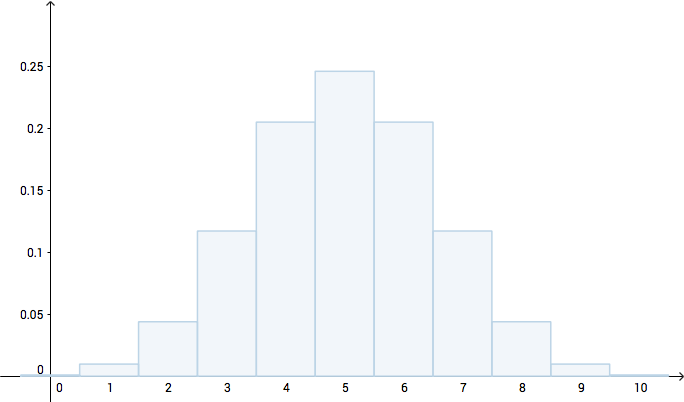
\includegraphics[width=0.5\textwidth]{fig/P_Value_Example_1.png}
\end{figure}
我扔了十次之后得到的结果是,有八次正面:
\begin{figure}[H]
    \centering
    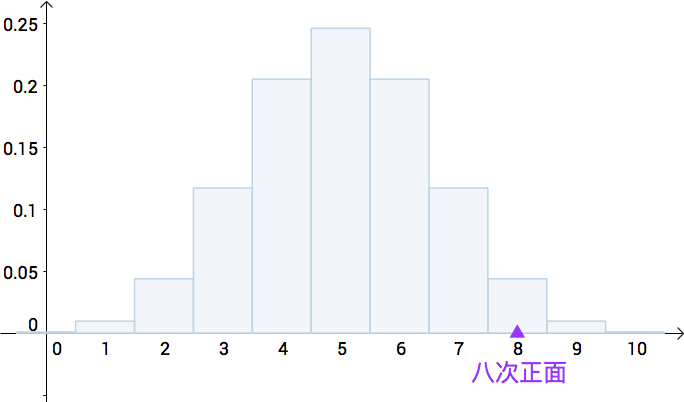
\includegraphics[width=0.5\textwidth]{fig/P_Value_Example_2.png}
\end{figure}

这个时候有个数学大佬出来定义了一个称为 P 值(p-value)的概念。把八次正面的概率,与更极端的九次正面、十次正面的概率加起来,得到的就是单侧P值:
$$
\text{p-value} = P(8 \le X \le 10) = 0.05
$$

其实,出现两次正面、一次正面、零次正面的概率也是很极端的,对应双侧P值:
$$
\text{p-value} = P(0 \le X \le 2)  +  P(8 \le X \le 10) = 0.1
$$

\subsection{显著水平}
总共扔10次硬币,那么是出现7次正面之后,可以认为“硬币是不公平的”,还是9次正面之后我才能确认“硬币是不公平的”,这是一个较为主观的标准。我们一般认为
$$
\text{p-value} \le 0.05
$$
就可以认为假设是不正确的。

0.05这个标准就是\textbf{显著水平},当然选择多少作为显著水平也是主观的。

比如,上面的扔硬币的例子,如果取单侧P值,那么根据我们的计算,如果扔10次出现9次正面:
$$
\text{p-value} = P(9 \le X \le 10) = 0.01 \le 0.05
$$

我们可以认为刚开始的假设错的很“显著”,也就是“硬币是不公平的”。

如果扔10次出现出现8次正面:
$$
\text{p-value} = P(8 \le X \le 10) = 0.05 \le 0.05
$$
这个和我们的显著水平是一样的,我们也可以拒绝假设,只是没有那么“显著”了。

\subsection{置信区间}
置信区间,就是一种区间估计。

\begin{framed}
点估计与区间估计:

以前很流行一种刮刮卡,游戏规则是(假设只有一个大奖):(1) 大奖事先就固定好了,一定印在某一张刮刮卡上;(2) 买了刮刮卡之后,刮开就知道自己是否中奖。

那么我们起码有两种策略来刮奖:(1) \textbf{点估计}:买一张,这就相当于你猜测这一张会中奖;(2) \textbf{区间估计}:买一盒,这就相当于你猜测这一盒里面会有某一张中奖

很显然区间估计的命中率会更高(当然费用会更高,因为风险降低了)。
\end{framed}

\subsubsection{一个例子}
对于人类真实的平均身高,我们是没有办法知道的,因为几乎不可能把每个人都统计到。但这个数据肯定是真实存在的,我们可以说,上帝知道。在这里我们引入了上帝视角,即上帝看到的人类身高的真实分布。假设人类的身高分布服从如下正态分布($\mu = 145, \sigma = 1.4$):
$$
X \sim N(145, 1.4^2)
$$

也就是说全体人类的平均身高为145cm,为了表示只有上帝可以看到,我把真实分布用虚线来表示:
\begin{figure}[H]
    \centering
    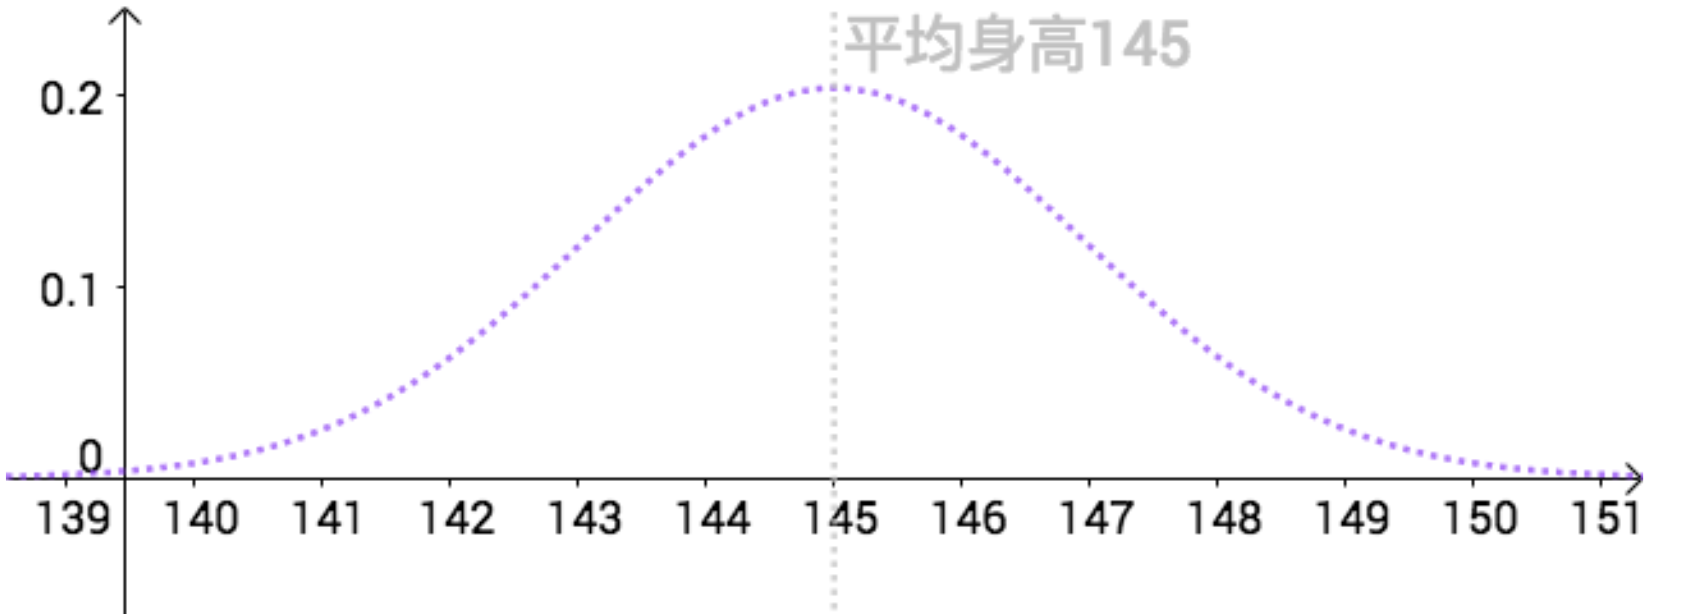
\includegraphics[width=0.5\textwidth]{fig/Confidence_Interval_Example_1.png}
\end{figure}

\subsubsection{点估计}
作为愚蠢的人类,我们只能在人群中抽样统计。比如得到一组抽样数据,我把算出来的样本均值(记作 $\hat{\mu}$ )画在图上(蓝色的点):
\begin{figure}[H]
    \centering
    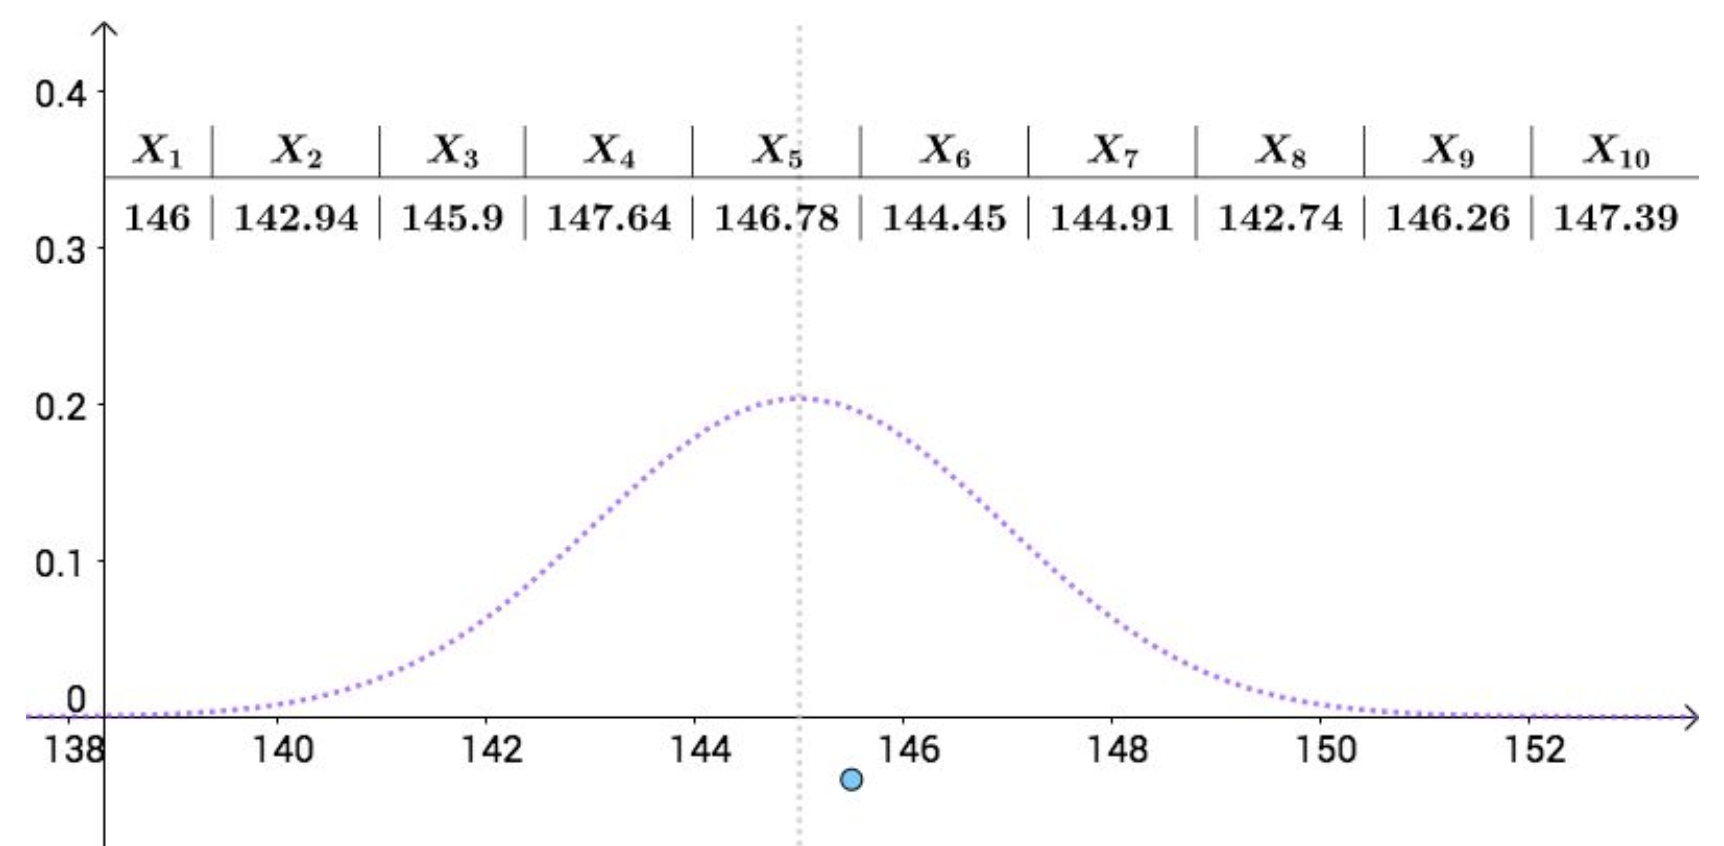
\includegraphics[width=0.5\textwidth]{fig/Confidence_Interval_Example_2.png}
\end{figure}

$\hat{\mu}$ 就是对真实的 $\mu$ 的一次点估计。

通过一次次的抽样,我们可以算出不同的身高均值的点估计:
\begin{figure}[H]
    \centering
    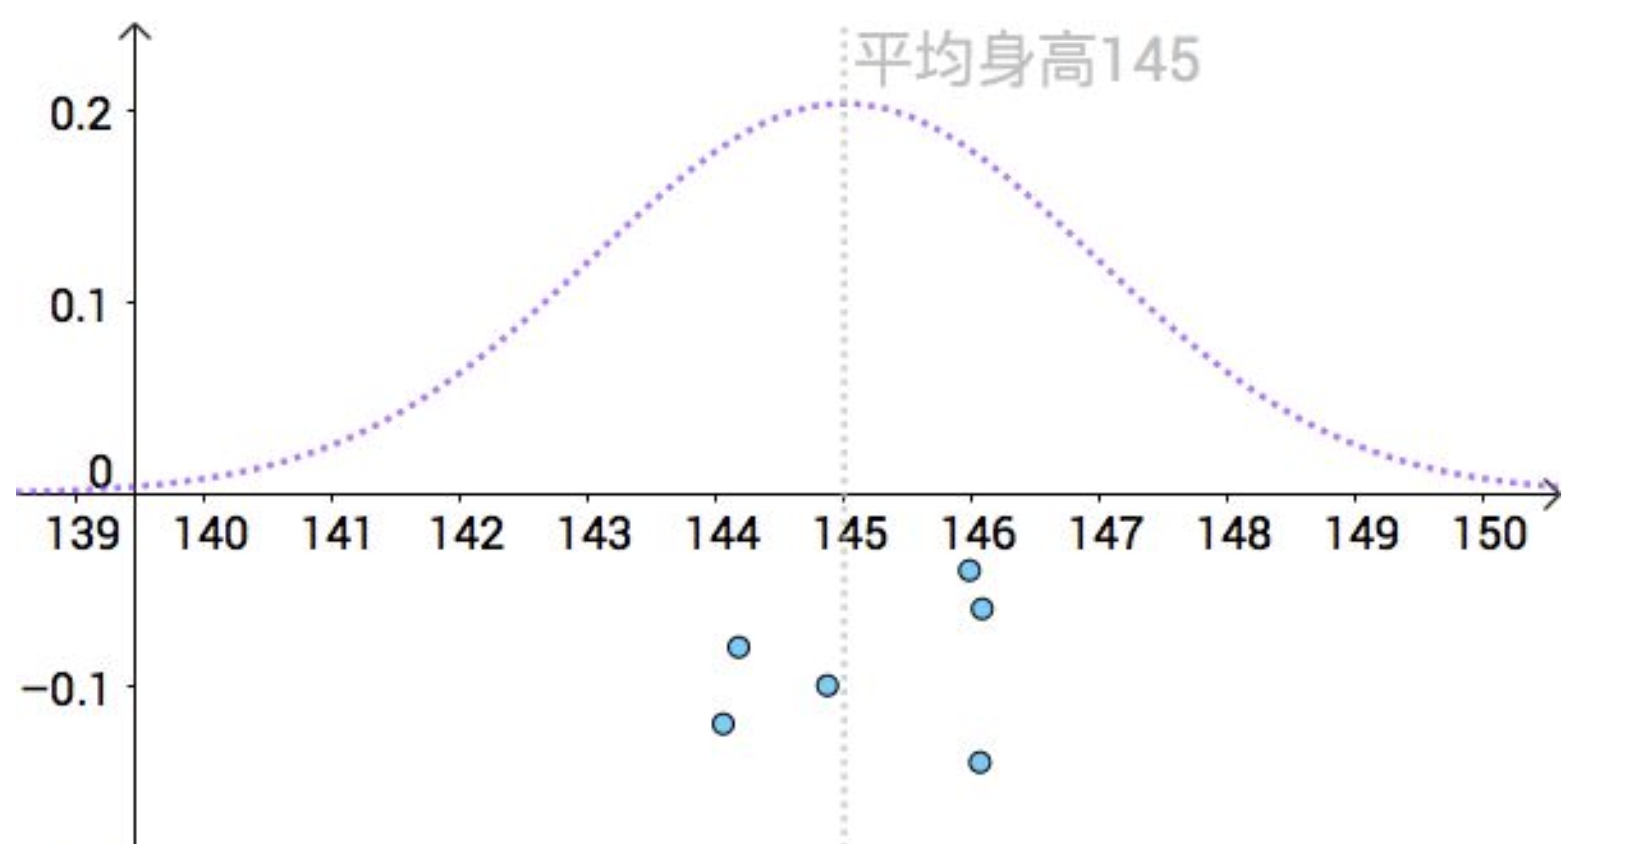
\includegraphics[width=0.5\textwidth]{fig/Confidence_Interval_Example_3.png}
\end{figure}

如果我们关闭上帝视角,我们分辨不出哪个点估计更好:
\begin{figure}[H]
    \centering
    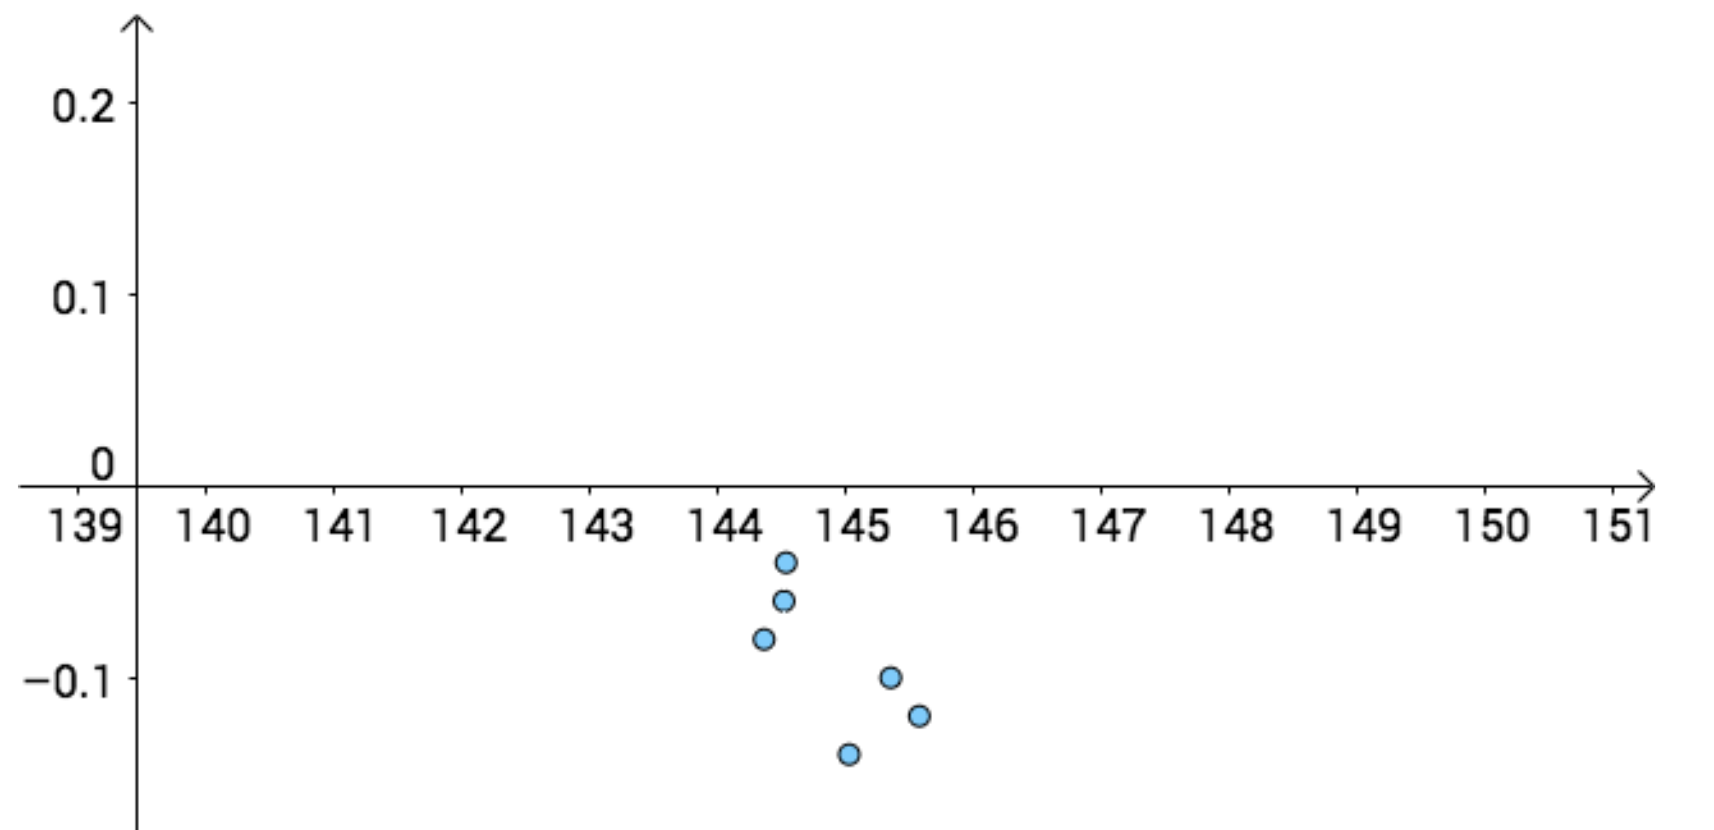
\includegraphics[width=0.5\textwidth]{fig/Confidence_Interval_Example_4.png}
\end{figure}
区间估计可以改进此问题。

\subsubsection{置信区间}
置信区间,提供了一种区间估计的方法。

下面采用 $95\%$ 置信区间来构造区间估计(什么是 $95\%$  置信区间,这个我们后面解释):
\begin{figure}[H]
    \centering
    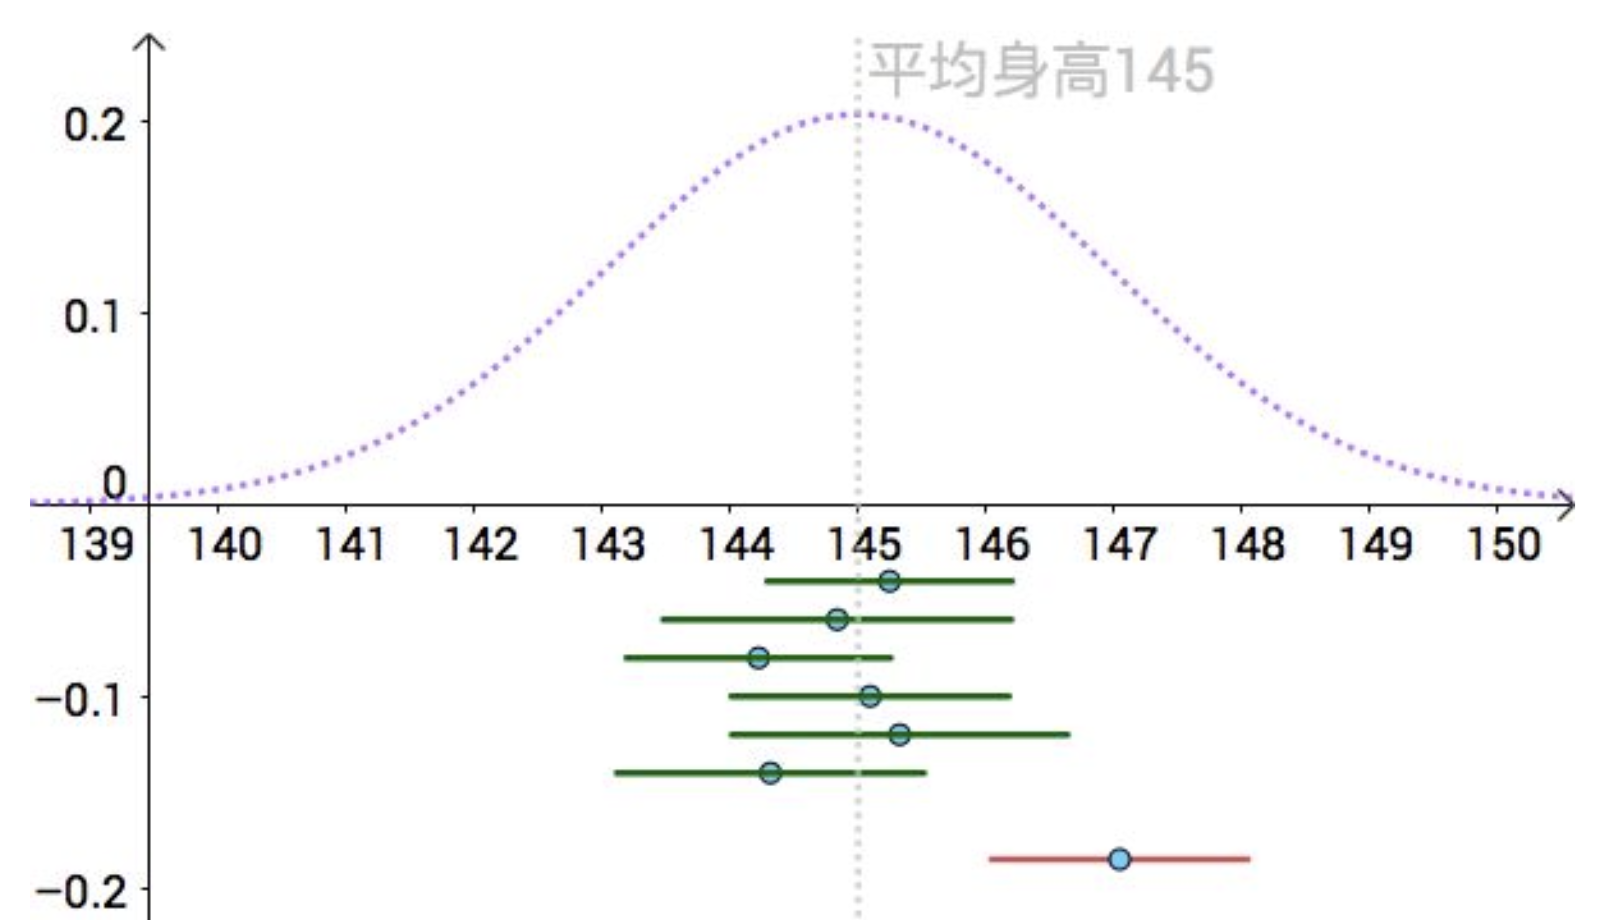
\includegraphics[width=0.5\textwidth]{fig/Confidence_Interval_Example_5.png}
\end{figure}

通过 $95\%$ 置信区间构造出来的区间,我们可以看到,基本上都包含了真实的 $\mu$,除了红色的那根。

关闭上帝视角,我们仍然不知道哪一个区间估计更好:
\begin{figure}[H]
    \centering
    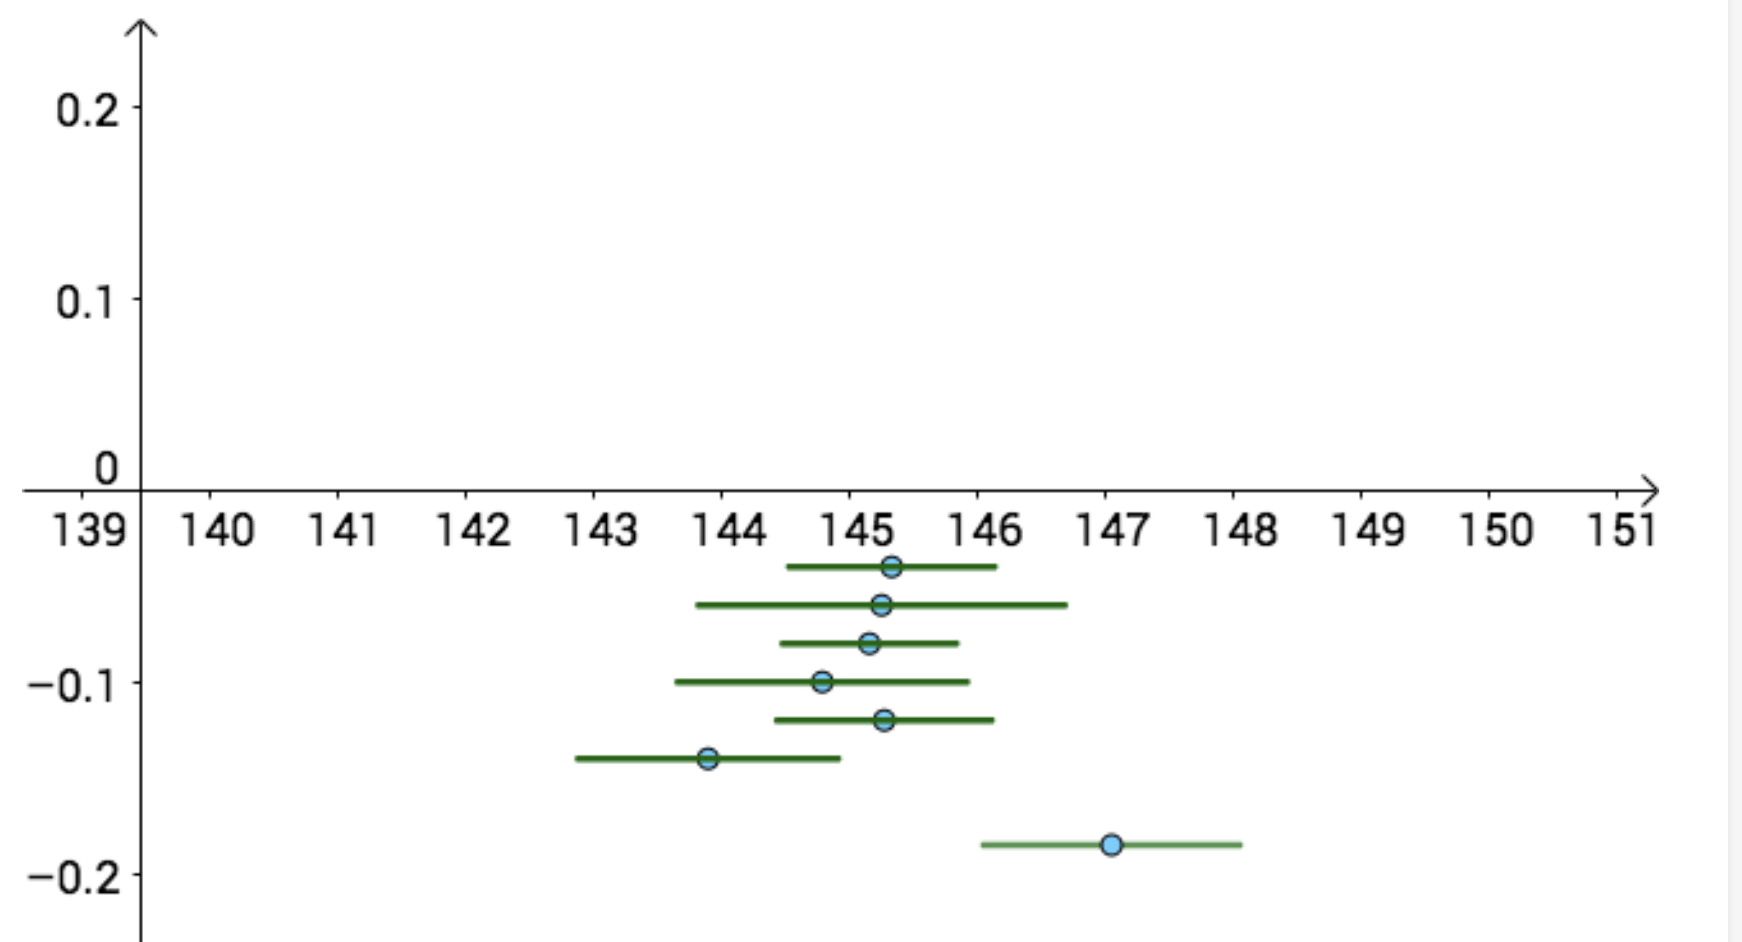
\includegraphics[width=0.5\textwidth]{fig/Confidence_Interval_Example_6.png}
\end{figure}

但是,和点估计比较:
\begin{itemize}
\setlength{\itemsep}{0pt}
\setlength{\parsep}{0pt}
\setlength{\parskip}{0pt}
    \item 点估计和区间估计,都不知道哪个点或者哪个区间更好;
    \item 但是,按照 $95\%$ 置信区间构造出来的区间,如果我构造出100个这样的区间,其中大约有95个会包含 $\mu$;
\end{itemize}

剩下的问题就是 $95\%$ 置信区间是如何构造的。

\subsubsection{ $95\%$ 置信区间}
假设人群的身高服从:
$$
X \sim N(\mu, \sigma^2)
$$

其中  $\mu$ 未知, $\sigma$ 已知。

我们不断对人群进行采样,样本的大小为 $n$,样本的均值:
$$
M = \frac{X_1 + X_2 + \cdots + X_n}{n}
$$

根据大数定律和中心极限定律, $M$ 服从:
$$
M \sim N(\mu, \frac{\sigma^2}{n})
$$

我们可以算出以 $\mu$ 为中心,面积为0.95的区间,如下图
\begin{figure}[H]
    \centering
    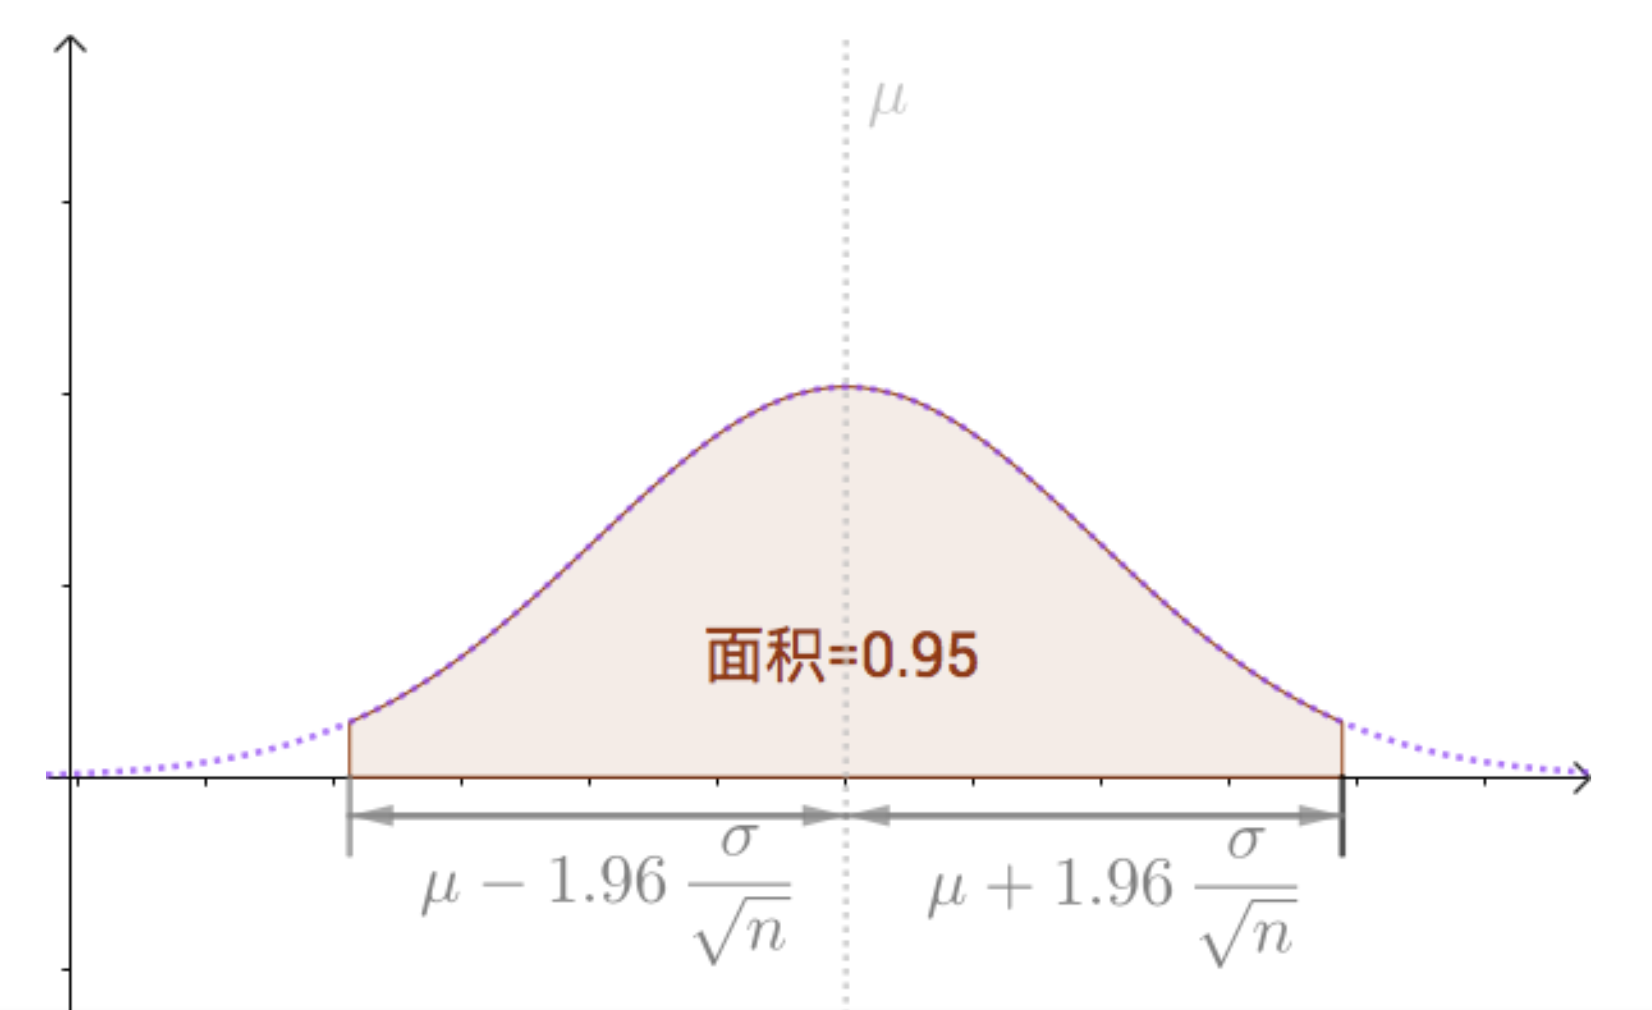
\includegraphics[width=0.5\textwidth]{fig/Confidence_Interval_Example_7.png}
\end{figure}

即:
$$
P(\mu - 1.96\frac{\sigma}{\sqrt{n}} \le M \le \mu + 1.96\frac{\sigma}{\sqrt{n}}) = 0.95
$$

也就是,$M$ 有 $95\%$  的几率落入此区间:
\begin{figure}[H]
    \centering
    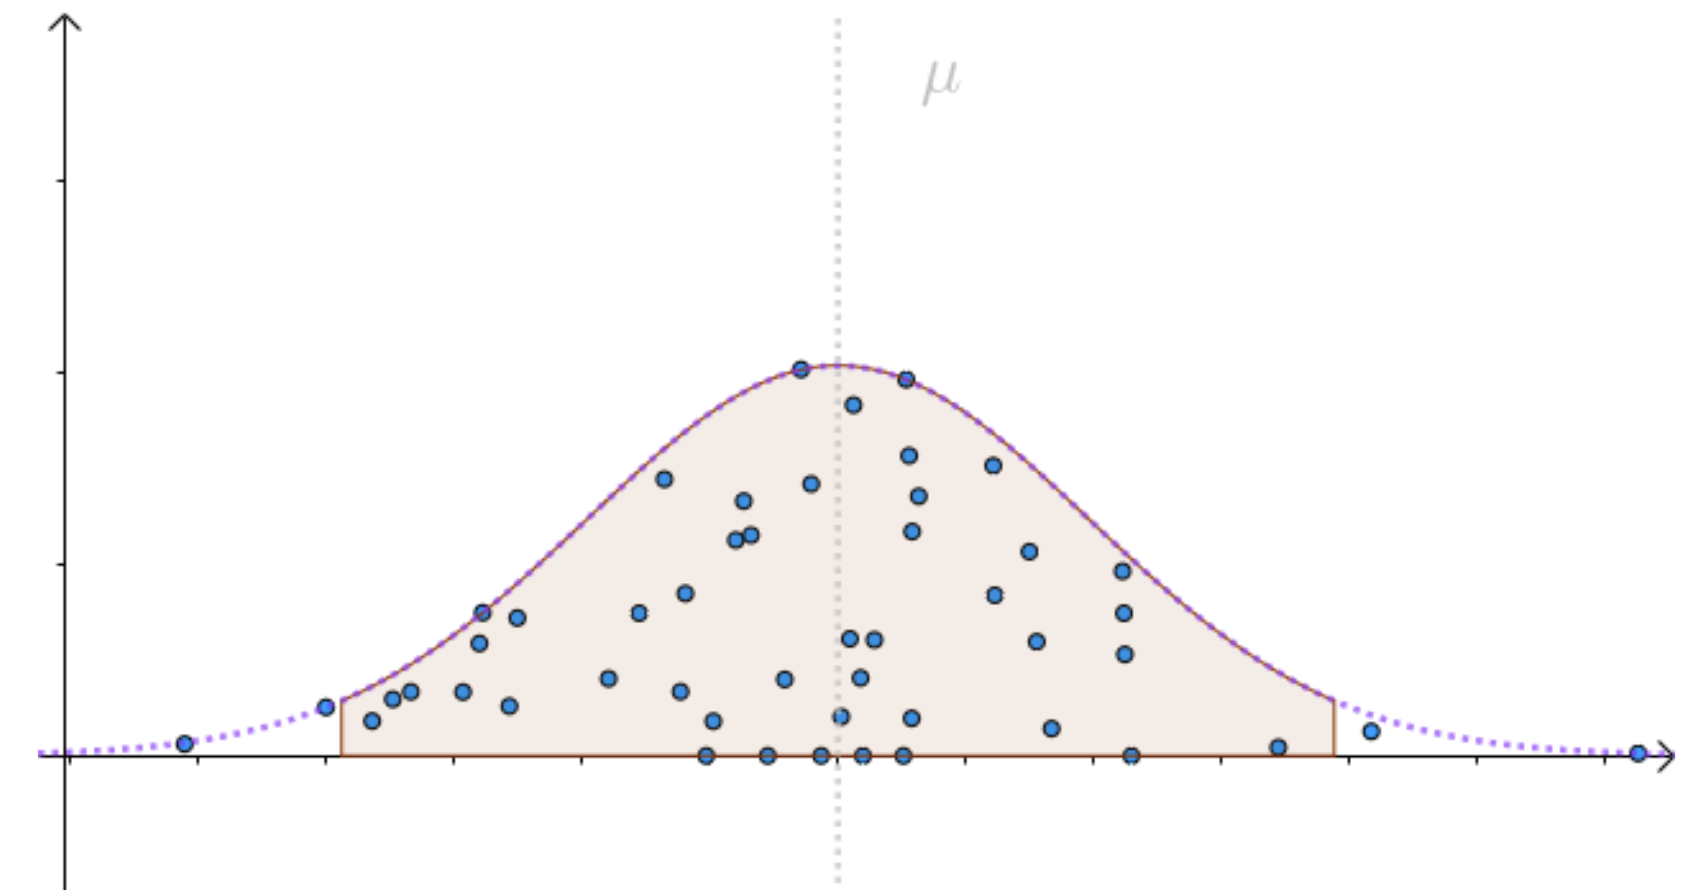
\includegraphics[width=0.5\textwidth]{fig/Confidence_Interval_Example_8.png}
\end{figure}

我们以 $1.96\frac{\sigma}{\sqrt{n}}$ 为半径做区间,就构造出了  $95\%$ 置信区间。按这样去构造的100个区间,其中大约会有95个会包含 $\mu$。

那么,只有一个问题了,我们不知道、并且永远都不会知道真实的 $\mu$ 是多少。我们就只有用$\hat{\mu}$ 来代替$\mu$:
$$
P(\hat{\mu} - 1.96\frac{\sigma}{\sqrt{n}} \le M \le \hat{\mu} + 1.96\frac{\sigma}{\sqrt{n}}) \approx 0.95
$$

\subsubsection{总结}
\begin{itemize}
\setlength{\itemsep}{0pt}
\setlength{\parsep}{0pt}
\setlength{\parskip}{0pt}
    \item 置信区间要求估计量是个常数;
    \item $95\%$ 也被称为置信水平,是统计中的一个习惯,可以根据应用进行调整。
\end{itemize}

\subsection{假设检验与与置信区间的关系}
置信区间,目的是根据样本构造一个区间,然后希望这个区间可以把真值包含进去,但是并不知道这个真值是多少;而假设检验,则是假设真值是多少,然后检验这个假设是否可能为真。

之所以觉得它们有关系,大概是因为它们都提到了0.05(比如之置信区间 95\%)。它们之间的关系也简单,如果我们提出来的假设 $\mu_0$ 在样本 $\bar{x}$ 的置信区间内,就可以通过测试
:
\begin{figure}[H]
    \centering
    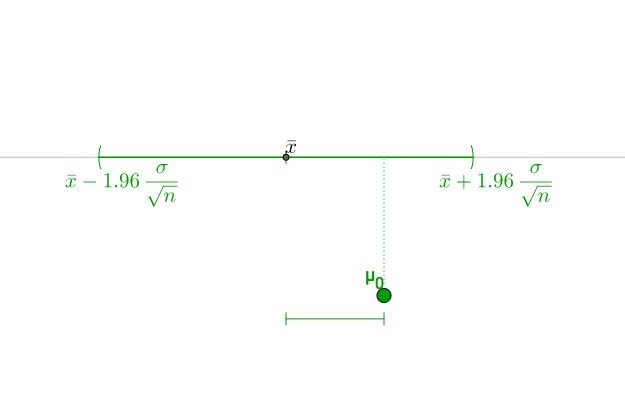
\includegraphics[width=0.5\textwidth]{fig/P_Value_Confidential_Example_1.jpg}
\end{figure}

反之,就不能通过:
\begin{figure}[H]
    \centering
    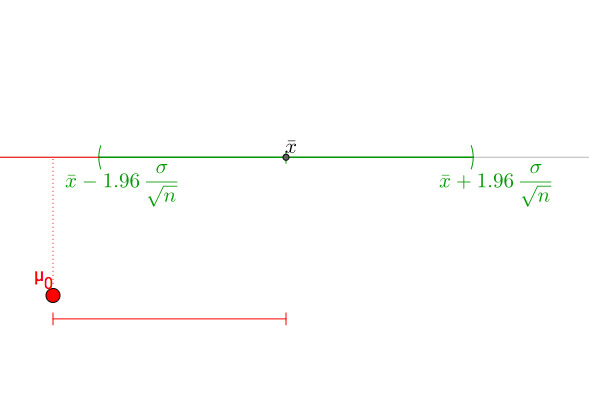
\includegraphics[width=0.5\textwidth]{fig/P_Value_Confidential_Example_2.png}
\end{figure}

\section{离线评估的主要方法\cite{Deep_Learning_Recommender_System}}
\subsection{Holdout 检验}
将原始样本随机划分为测试集和验证集两部分;比如,可以将样本按照70\%-30\%的比例随机分成两部分,70\%的样本用于模型的训练,30\%的样本用于模型的评估

Holdout 检验的缺点:在验证集上计算出来的评估指标与训练集和验证集的划分有很大关系,如果仅仅进行少量 holdout 检验,则得到的结论存在较大的随机性。为了消除这种随机性,“交叉检验”的思想被提出。

\subsection{交叉检验}
\subsubsection{k-fold 交叉检验}
先将全部样本划分为$k$个大小相等的样本子集;依次遍历这$k$个子集,每次都把当前子集作为验证集,其余所有子集作为训练集,进行模型的训练和评估;最后将所有$k$次的评估指标的平均值作为最终的评估指标。在实际实验中,$k$经常取10。

\subsubsection{留一验证}
每次留下一个样本作为验证集,其余所有样本作为训练集。样本总数为$n$,依次遍历所有$n$个样本,进行$n$次验证,再讲评估指标求平均得到最终各指标。在样本总数较多的情况下,留一验证法的时间开销极大。事实上,留一验证是留$p$验证的特例。留$p$验证是指每次留下$p$个样本作为验证集,而从$n$个元素中选择$p$个元素有$C_n^p$中可能,因此它的时间开销远远大于留一验证,因此很少在实际工程中应用。

\subsubsection{自助法(bootstrap)}
不管是 holdout 检验还是交叉检验,都是基于划分样本机和验证集的方式进行模型评估的。然而,当样本规模比较小时,将样本机进行划分会让训练集进一步减小,这可能会影响模型的训练效果。

bootstrap 法能在一定程度上维持训练集样本的规模。是基于自助采样法的验证方法:对于总数为$n$的样本集合,进行$n$次有放回的随机抽样,得到大小为$n$的训练集。在$n$次采样过程中,有的样本会被重复采样,有的样本没有被抽出过,将这些没有被抽出的样本作为验证集进行模型验证,就是自助法的验证过程。

\section{Netflix推荐系统模型的快速线上评估方法——Interleaving\cite{Interleaving_In_Netflix}}
周所周知,Netflix是美国的流媒体巨头,其广为人知的原因不仅是因为其多部知名的原创剧,高昂的市值,在推荐技术领域,Netflix也一直走在业界的最前沿。那么驱动Netflix实现推荐系统快速迭代创新的重要技术,就是我们今天要介绍的快速线上评估方法——Interleaving。

\subsection{Netflix推荐系统问题背景}
Netflix几乎所有页面都是推荐算法驱动的,每种算法针对不同的推荐场景进行优化。 例如,主页上的“Top Picks行”根据视频的个性化排名提供推荐,而“Trending Now行”包含了最近的流行趋势。 这些个性化的行共同构成了Netflix将近1亿会员“千人千面“的个性化主页。

对于强算法驱动的Netflix来说,算法的迭代创新当然是必不可少的。为了通过算法最大化Netflix的商业目标(这些商业指标包括每月用户订阅数、观看总时长等等),需要进行大量的AB Test来验证新算法能否有效提升这些关键的产品指标。

这就带来一个矛盾,就是\textbf{算法工程师们日益增长的AB Test需求和线上AB Test资源严重不足之间的矛盾}。因为线上AB Test必然要占用宝贵的线上流量资源,还有可能会对用户体验造成损害,但线上流量资源显然是有限的,而且只有小部分能够用于AB Test;而算法研发这侧,算法驱动的使用场景不断增加,大量候选算法需要逐一进行AB Test。这二者之间的矛盾必然愈演愈烈。这就迫切需要设计一个快速的线上评估方法。

为此,Netflix设计了一个两阶段的线上测试过程(如图2)。

(1). \textbf{第一阶段利用被称为Interleaving的测试方法进行候选算法的快速筛选,从大量初始想法中筛选出少量“优秀的”Ranking算法}。

(2). \textbf{第二阶段是对缩小的算法集合进行传统的AB Test,以测量它们对用户行为的长期影响}。

\begin{figure}[H]
    \centering
    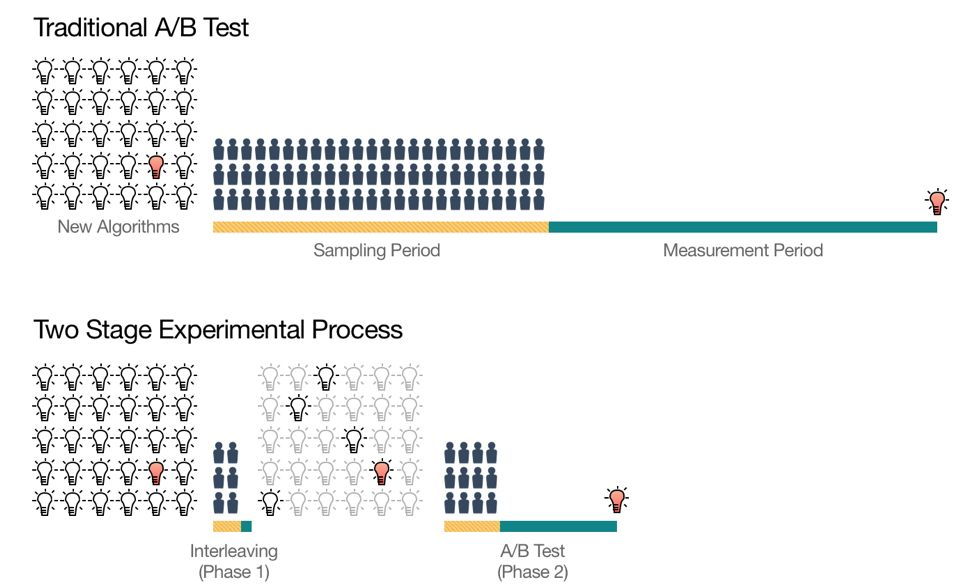
\includegraphics[width=1\textwidth]{fig/Netflix_Interleaving_Idea.jpg}
    \caption*{图2:使用Inter leaving进行快速线上测试。 用灯泡代表候选算法。 其中,最优的获胜算法用红色表示。Interleaving能够快速地将最初的候选算法集合进行缩减,相比传统的AB Test更快地确定最优算法。}
\end{figure}

\subsection{传统AB Test存在的问题}
传统的AB Test除了存在效率问题,还存在一些统计学上的显著性差异问题。下面用一个很典型的AB Test问题来进行说明。

这里设计一个AB Test来验证用户群体是否对“可口可乐”和“百事可乐”存在口味倾向。那么按照传统的做法,我们会将测试人群随机分成两组然后进行“盲测”,即在不告知可乐品牌的情况下进行测试。第一组只提供可口可乐,第二组只提供百事可乐,然后根据大家一定时间内的可乐消耗量来观察人们是更喜欢“可口可乐”还是“百事可乐”。

这个实验一般意义上确实是有效的,很多时候我们也是这么做的。但也确实存在一些潜在的问题:

\begin{itemize}
\setlength{\itemsep}{0pt}
\setlength{\parsep}{0pt}
\setlength{\parskip}{0pt}
    \item 总的测试人群中,对于可乐的消费习惯肯定各不相同,从几乎不喝可乐到每天喝大量可乐的人都有;
    \item 可乐的重消费人群肯定只占总测试人群的一小部分,但他们可能占整体汽水消费的较大比例;
\end{itemize}

这两个问题导致了,即使\textbf{AB两组之间重度可乐消费者的微小不平衡也可能对结论产生不成比例的影响}。

在互联网场景下,这样的问题同样存在。比如Netflix场景下,非常活跃用户的数量是少数,但其贡献的观看时长却占较大的比例,因此Netflix AB Test中活跃用户被分在A组的多还是被分在B组的多,将对结果产生较大影响,从而掩盖模型的真实效果。

那么如何解决这个问题呢?一个方法是不对测试人群进行分组,而是让所有测试者都可以自由选择百事可乐和可口可乐(测试过程中仍没有品牌标签,但能区分是两种不同的可乐)。在实验结束时,统计每个人可口可乐和百事可乐的消费比例,然后进行平均后得到整体的消费比例。

这个测试方案的优点在于:
\begin{itemize}
\setlength{\itemsep}{0pt}
\setlength{\parsep}{0pt}
\setlength{\parskip}{0pt}
    \item \textbf{消除了AB组测试者自身属性分布不均的问题;}
    \item \textbf{通过给予每个人相同的权重,降低了重度消费者对结果的过多影响。}
\end{itemize}

\subsection{Netflix的快速线上评估方法——Interleaving}
图3描绘了AB Test和Interleaving之间的差异。
\begin{itemize}
\setlength{\itemsep}{0pt}
\setlength{\parsep}{0pt}
\setlength{\parskip}{0pt}
    \item 在传统的AB Test中,Netflix会选择两组订阅用户:一组接受Ranking算法A的推荐结果 ,另一组接受Ranking算法B的推荐结果。
    \item 在Interleaving测试中,只有一组订阅用户,这些订阅用户会接受到通过混合算法A和B的排名生成的交替排名。
\end{itemize}

这就使得用户同时可以在一行里同时看到算法A和B的推荐结果(用户无法区分一个item是由算法A推荐的还是算法B推荐的)。进而可以通过计算观看时长等指标来衡量到底是算法A好还是算法B好。
\begin{figure}[H]
    \centering
    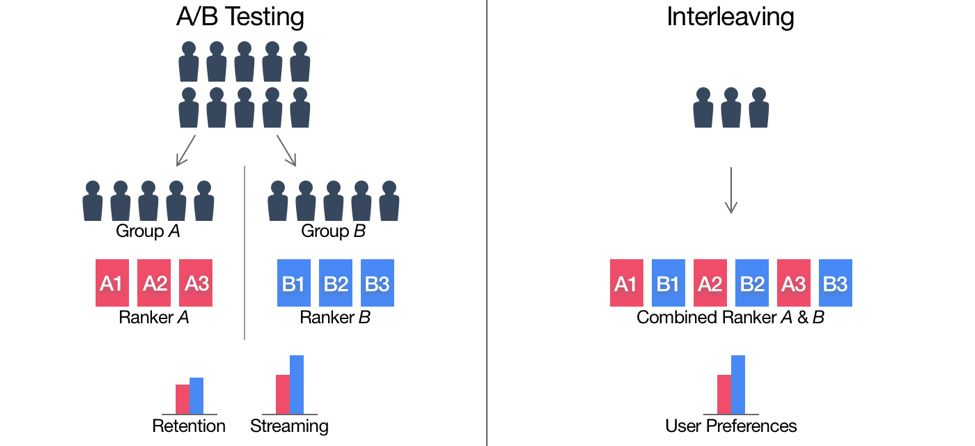
\includegraphics[width=1\textwidth]{fig/Netflix_Interleaving_Vs_AB_Test.jpg}
    \caption*{图3:传统AB Test和Interleaving 在传统AB Test中,测试用户分为两组,一组暴露于排名算法A ,另一组暴露于算法B,在两组之间进行比较观看时长	等核心评估指标。另一方面,Interleaving将所有测试用户暴露于算法A和B的混合排名,再比较算法相对应的item的指标}
\end{figure}

当然,在用Interleaving方法进行测试的时候,必须要考虑位置偏差的存在,避免来自算法A的视频总排在第一位。因此需要以相等的概率让算法A和算法B交替领先。这类似于在野球场打球时,两个队长先通过扔硬币的方式决定谁先选人,然后在交替选队员的过程。

在清楚了Interleaving方法之后,还需要验证这个评估方法到底能不能替代传统的AB Test,会不会得出错误的结论。Netflix从两个方面进行了验证,一是Interleaving的“灵敏度”,二是Interleaving的“正确性”。

\subsection{Interleaving与传统AB Test的灵敏度比较}
Netflix的这组实验希望验证的是Interleaving方法相比传统AB Test,\textbf{需要多少样本就能够验证出算法A和算法B的优劣}。我们之前一再强调线上测试资源的紧张,因此这里自然希望Interleaving能够利用较少的线上资源,较少的测试用户就解决评估问题。这就是所谓的“灵敏度比较”。

图5是实验结果,横轴是参与实验的样本数量,纵轴Netflix没有给出非常精准的解释,但我们可以理解为是判定算法A是否比算法B好的“错误”概率。可以看出的是interleaving的方法利用$10^3$个样本就能够判定算法A是否比B好,而AB test则需要$10^5$个样本才能够将错误率降到5\%以下。这就意味着利用一组AB Test的资源,我们可以做100组Interleaving实验。这无疑大大加强了线上测试的能力。

\begin{figure}[H]
    \centering
    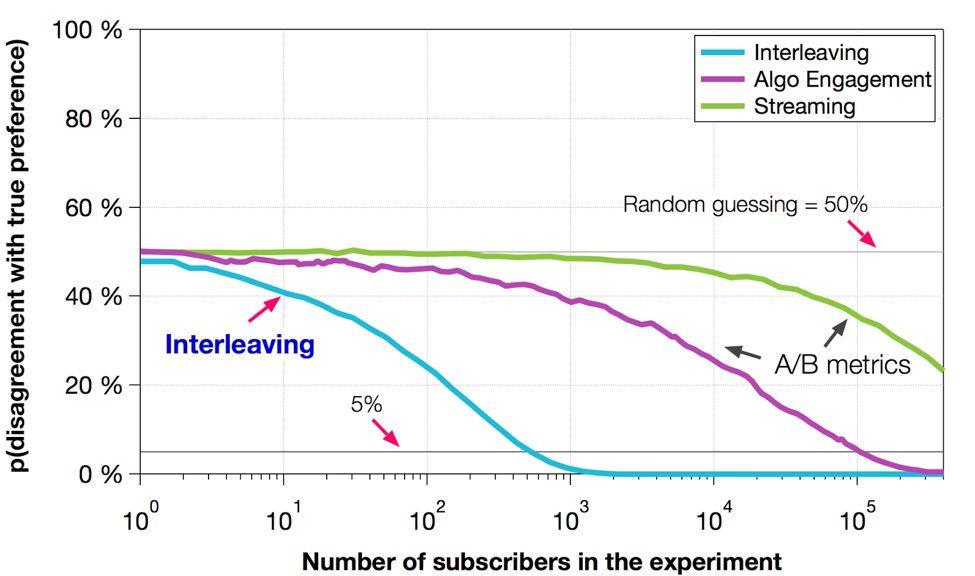
\includegraphics[width=1\textwidth]{fig/Netflix_Interleaving_Vs_AB_Test_Result.jpg}
    \caption*{图5:对Interleaving与传统AB Test指标的灵敏度。 与最敏感的AB Test指标相比,Interleaving也只需要1/100的订阅用户样本就能够确定用户更偏爱哪个算法}
\end{figure}

\subsection{Interleaving指标与AB Test指标的相关性}
除了能够利用小样本快速进行算法评估外,Interleaving的判断结果是否与AB Test一致,也是检验Interleaving能否在线上评估第一阶段取代AB Test的关键。

图6显示了Interleaving中的实验指标与AB Test指标之间的相关性。每个数据点代表一个Ranking算法。 我们发现Interleaving指标与AB Test评估指标之间存在非常强的相关性,这就验证了在Interleaving实验中胜出的算法也极有可能在之后的AB Test中胜出。
\begin{figure}[H]
    \centering
    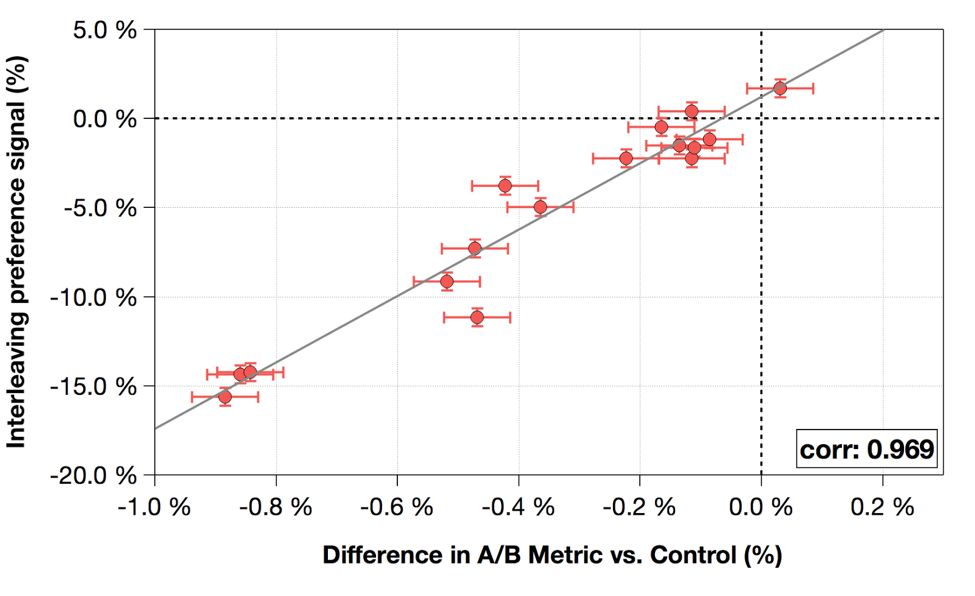
\includegraphics[width=1\textwidth]{fig/Netflix_Interleaving_Vs_AB_Test_Relation.jpg}
    \caption*{图6:Interleaving指标与AB Test指标的相关性。 每个点表示一个Ranking算法的实验结果。 Interleaving指标与AB Test指标存在很强的相关性}
\end{figure}

\subsection{结论}
通过实验我们已经知道Interleaving是一种强大快捷的算法验证方法,它加速了Netflix各类Ranking算法的迭代创新。

但我们也要清楚的是Interleaving方法也存在一定的局限性,主要是下面两点:
\begin{itemize}
\setlength{\itemsep}{0pt}
\setlength{\parsep}{0pt}
\setlength{\parskip}{0pt}
    \item \textbf{工程实现的框架较传统AB Test复杂}。由于Interleaving实验的逻辑和业务逻辑纠缠在一起,因此业务逻辑可能会被干扰。而且为了实现Interleaving,需要将大量辅助性的数据标示添加到整个数据pipeline中,这都是工程实现的难点;
    \item \textbf{Interleaving毕竟只是对用户对算法推荐结果偏好程度的相对测量,不能得出一个算法完整的表现}。比如我们想知道算法A能够将用户整体的观看时长提高多少,使用Interleaving是无法得出这样的结论的。为此Netflix才设计了Interleaving+AB Test两级实验结构,完善整个线上测试的框架。
\end{itemize}


%\printbibliography
\bibliography{../ref}
\bibliographystyle{IEEEtran}
\end{document}
